\section{Framework Design}

\subsection{Architecture Overview}

The proposed framework integrates three main components:
\begin{enumerate}
    \item \textbf{Perception Processing Layer}: Handles sensor data aggregation and context extraction
    \item \textbf{LLM Integration Layer}: Manages prompt generation and response processing
    \item \textbf{Human Interface Layer}: Provides natural language interaction capabilities
\end{enumerate}

\begin{center}
    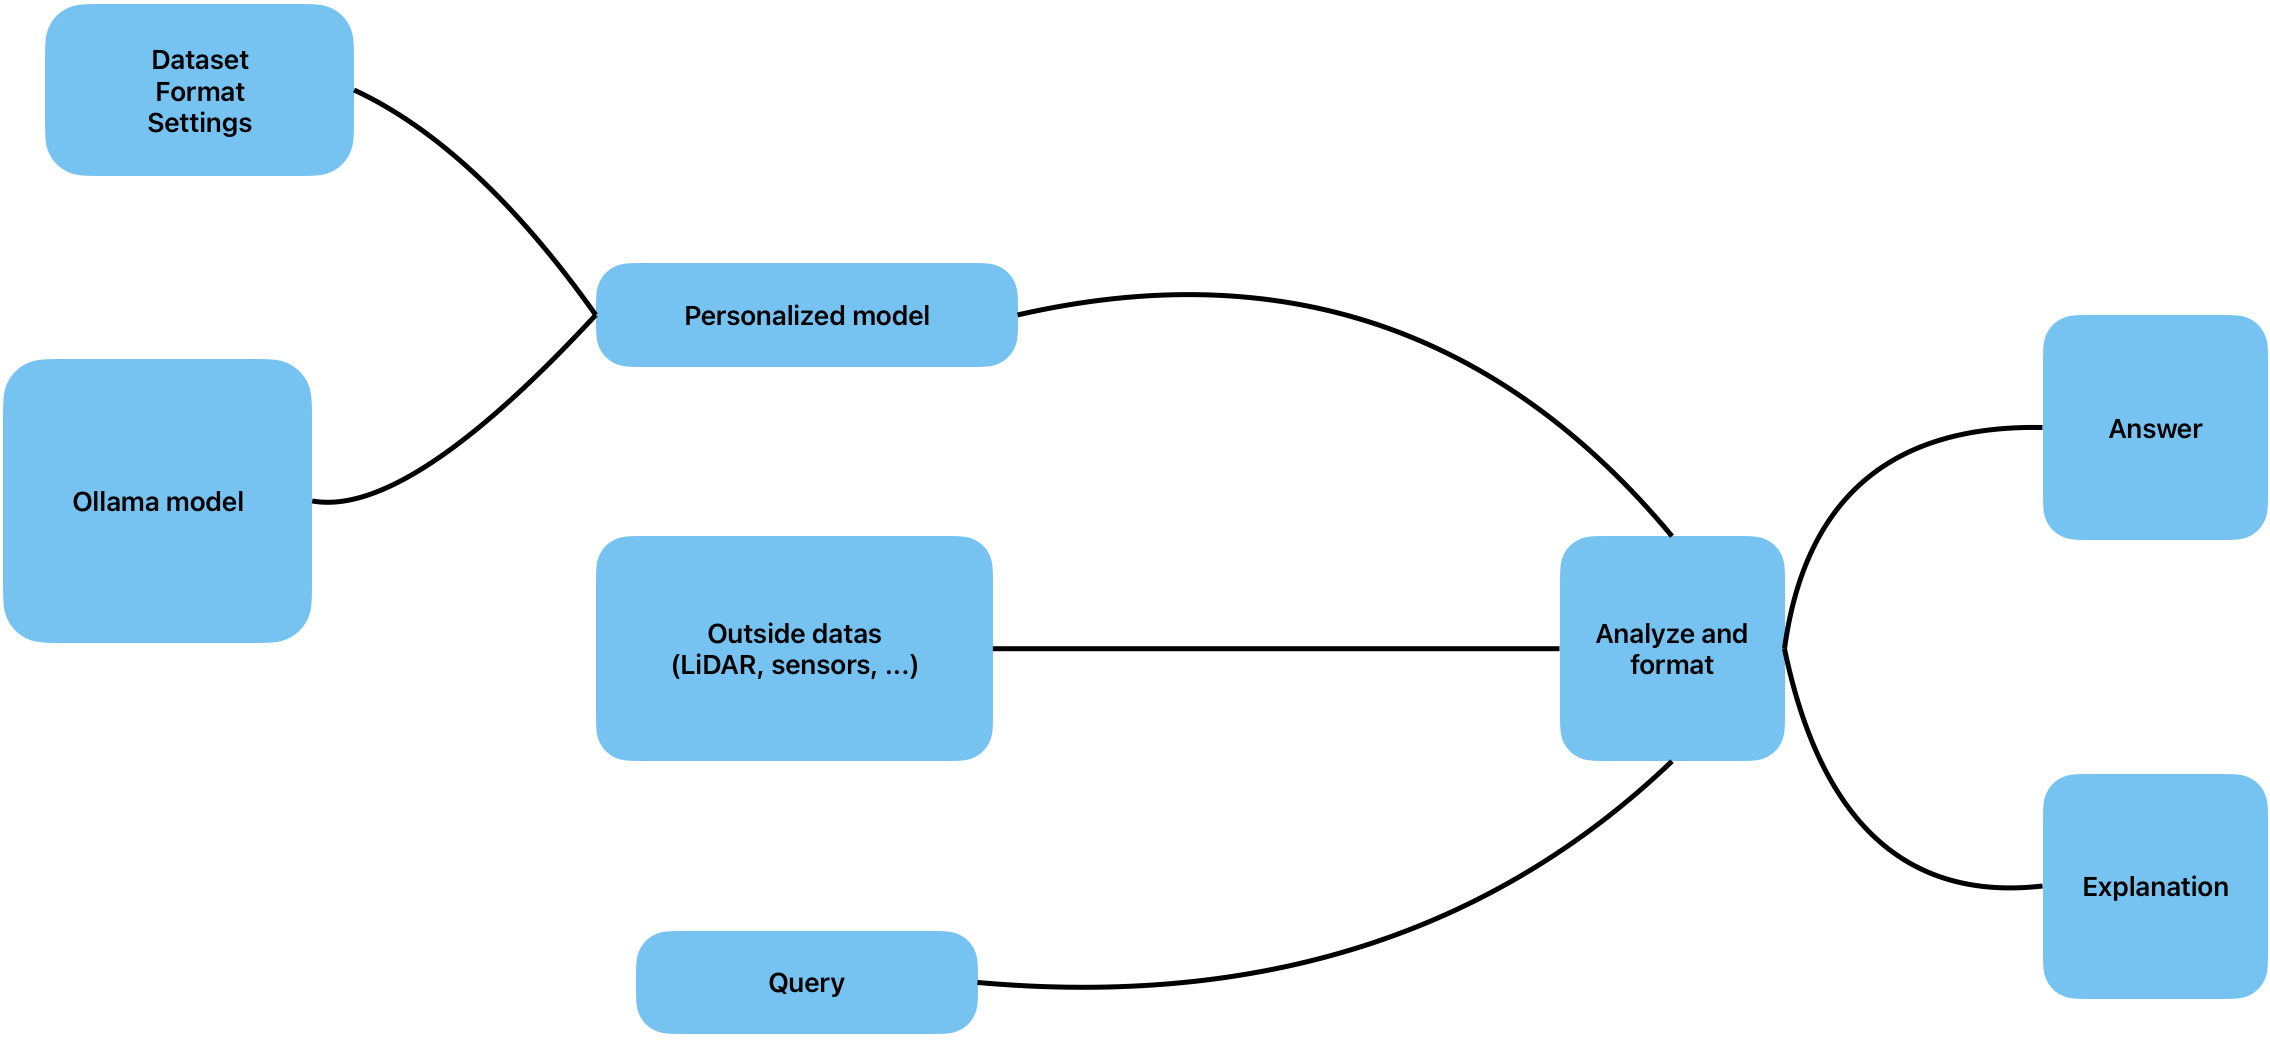
\includegraphics[scale=0.45]{figures/Model-HCI.png}
\end{center}

\subsection{Installation of the Project}

The project is designed to be easily deployable on any computer with minimal setup requirements. The following prerequisites are needed:

\begin{itemize}
    \item \textbf{Python 3.8+} (recommended: Python 3.11)
    \item \textbf{Ollama} - Local LLM server for model hosting
    \item \textbf{llama3.2} model or compatible LLM model
    \item \textbf{make} (optional, for automation)
    \item \textbf{git} for repository cloning
\end{itemize}

\subsubsection{Step-by-Step Installation Process}

\textbf{1. Repository cloning}

The project can be obtained from the GitHub repository:

\begin{verbatim}
    git clone https://github.com/Vlor999/HCI.git
    cd HCI
\end{verbatim}

\textbf{2. Ollama installation and setup}

Ollama serves as the local LLM server, providing the computational backend for natural language processing:

\begin{itemize}
    \item Download and install Ollama from \texttt{https://ollama.com/download}
    \item Start the Ollama server: \texttt{ollama serve}
    \item Pull the required model: \texttt{ollama pull llama3.2} (or any other model)
\end{itemize}

\textbf{3. Project environment setup}

The project uses automated setup through make commands:

\begin{verbatim}
    make init
    make install
\end{verbatim}

This process creates the necessary directory structure and installs Python dependencies in a virtual environment.

\textbf{4. Optional code formatting}

For development consistency:

\begin{verbatim}
    make format
\end{verbatim}
But if you also want to stay consistent with the all code you have to run the following command :
\begin{verbatim}
    pre-commit install
\end{verbatim}
Like that for the next commit that you'll do everything will be checked before you submit it.

\subsection{System execution}

\subsubsection{Running the Application}

The system can be launched using either automated make commands or direct Python execution:

\begin{verbatim}
    make run
\end{verbatim}

or manually:

\begin{verbatim}
    .venv/bin/python main.py
\end{verbatim}

Obviously you can add some CLI commands and if you are into the current env you can simply run :

\begin{verbatim}
    python main.py
\end{verbatim}

If you want to know all the commands that can be used try the help CLI argument.

\subsubsection{Testing Framework}

The project includes comprehensive testing capabilities:

\begin{verbatim}
    make test
\end{verbatim}

For coverage analysis with HTML reporting:

\begin{verbatim}
    make coverage
\end{verbatim}

The coverage report can be viewed by opening \texttt{htmlcov/index.html} in a web browser.

\subsection{Data flow and processing pipeline}

The system processes robot perception data through a structured pipeline:
\begin{itemize}
    \item Environmental/Weather context extraction from sensor readings
    \item Path analysis and decision point identification
    \item Prompt template generation with structured information
    \item LLM query processing and response generation
    \item Natural language explanation delivery to users
\end{itemize}


\subsection{Project structure and organization}

The framework follows a modular architecture with clear separation of concerns:

\begin{verbatim}
    src/           # Source code modules
    tests/         # Unit tests and test data
    data/          # Example path scenarios (JSON)
    log/           # Conversation logs (Markdown)
    doc/           # Documentation and roadmap
    evaluation/    # Evaluation scripts and results
    Makefile       # Automation commands
    requirements.txt # Python dependencies
\end{verbatim}

\subsection{Usage workflow}

The typical user interaction follows this pattern:
\begin{enumerate}
    \item The system displays current robot path and environmental context
    \item Users can ask multiple questions about path decisions and conditions
    \item The LLM processes queries and generates contextual explanations
    \item Sessions are terminated with \texttt{exit} or \texttt{quit} commands
    \item Conversation logs are automatically saved in Markdown format in the \texttt{log/} directory
\end{enumerate}

\subsection{Configuration and customization}

The system supports various customization options:

\begin{itemize}
    \item \textbf{Path scenarios}: Edit \texttt{data/paths.json} to add or modify navigation scenarios
    \item \textbf{LLM models}: The model name can be changed in the source code for different LLM variants
    \item \textbf{Logging}: Conversation logs are automatically generated and stored for analysis
\end{itemize}

\subsection{Technical requirements}

The framework is designed with several technical requirements in mind.
It must support real-time processing to enable interactive use and immediate responses to user queries.
The architecture should remain modular to facilitate adaptation across different robot platforms and allow for future extensions.
Scalability is also essential, ensuring that the system can handle a variety of explanation types and increasing complexity as needed.

\subsection{Troubleshooting and common issues}

When deploying the system, several common issues may arise. First, it is important to ensure that the Ollama server is running by verifying that the \texttt{ollama serve} command is active and that the required model has been properly pulled.
Port conflicts can also occur, as only one Ollama server instance should be running on port 11434 at any given time. Additionally, the Python environment must be correctly set up, make sure that the virtual environment (\texttt{.venv}) is properly activated before running any Python scripts.
Finally, confirm that the necessary large language model (LLM) is downloaded and accessible to avoid runtime errors related to model availability.
\subsection{Integration Capabilities}
